\documentclass[12pt,a4paper]{report}
\usepackage[utf8]{inputenc}
\usepackage[francais]{babel}
\usepackage[T1]{fontenc}
\usepackage{amsmath}
\usepackage{amsfonts}
\usepackage{amssymb}
\usepackage{graphicx}
\graphicspath{{pic/}}
\usepackage{authblk}
\author{Renan Husson, Quentin Rouland, Jerome Morjon, Matthieu Penchenat, Alexandre Pereira, Sébastien Bouyt}
\affil{Université Toulouse, Jean Jaurès - L3 MIASHS \\ Document D2 : Conceptio}
\begin{document}
\title{Projet Web - AJAX}
\maketitle
\renewcommand{\contentsname}{Sommaire}
\tableofcontents
\chapter*{Introduction}
\addcontentsline{toc}{chapter}{Introduction}
Animateur/Secrétaire : \\
02/02/2015 : Animateur : Sebastien Bouyt Secrétaire : Renan Husson \\
03/02/2015 : Animateur : Alexandre Pereira Secrétaire : Rouland Quentin


\chapter{Charte graphique}
\begin{figure}
	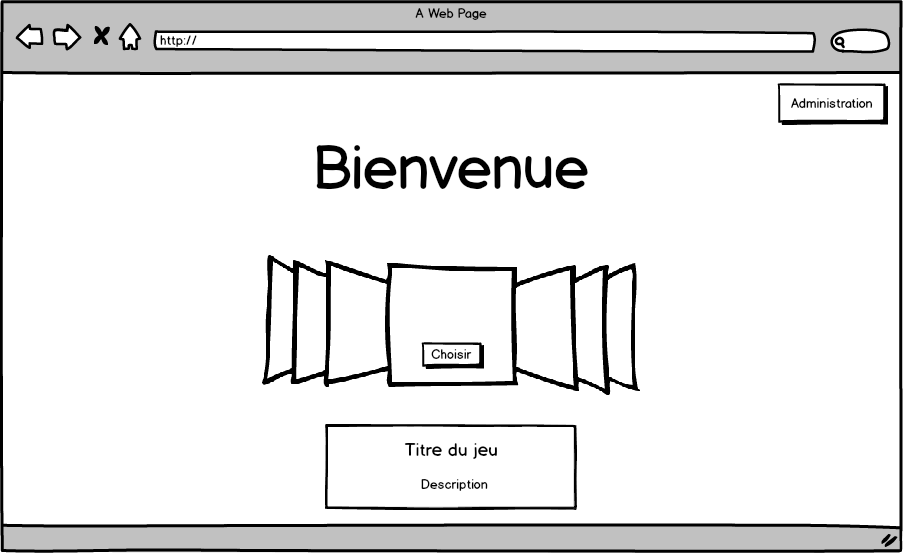
\includegraphics[width=350px]{../Maquette/Acceuil.png}
	\caption{Page d’accueil}
\end{figure}
\begin{figure}
	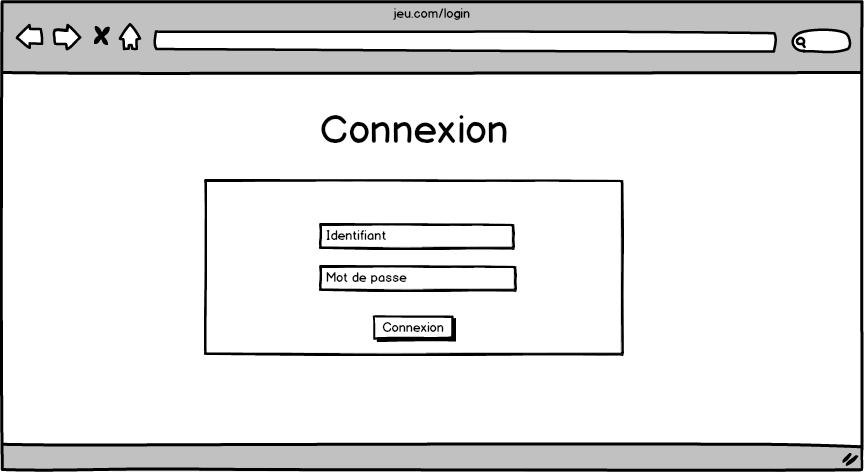
\includegraphics[width=350px]{../Maquette/Connexion.png}
	\caption{Page connexion}
\end{figure}
\begin{figure}
	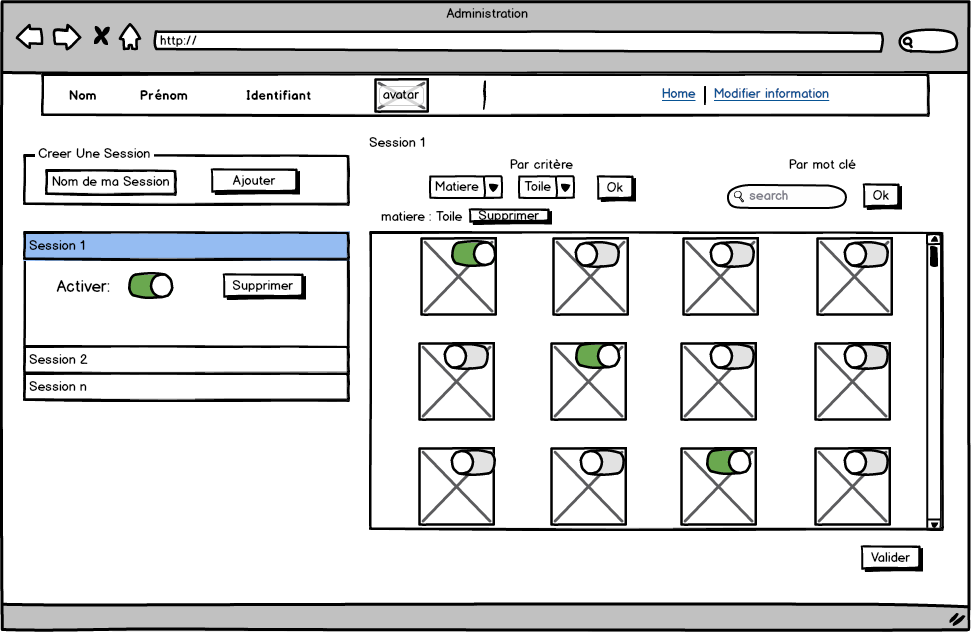
\includegraphics[width=350px]{../Maquette/adherent.png}
	\caption{Page de gestion de session par un référent}
\end{figure}
\begin{figure}
	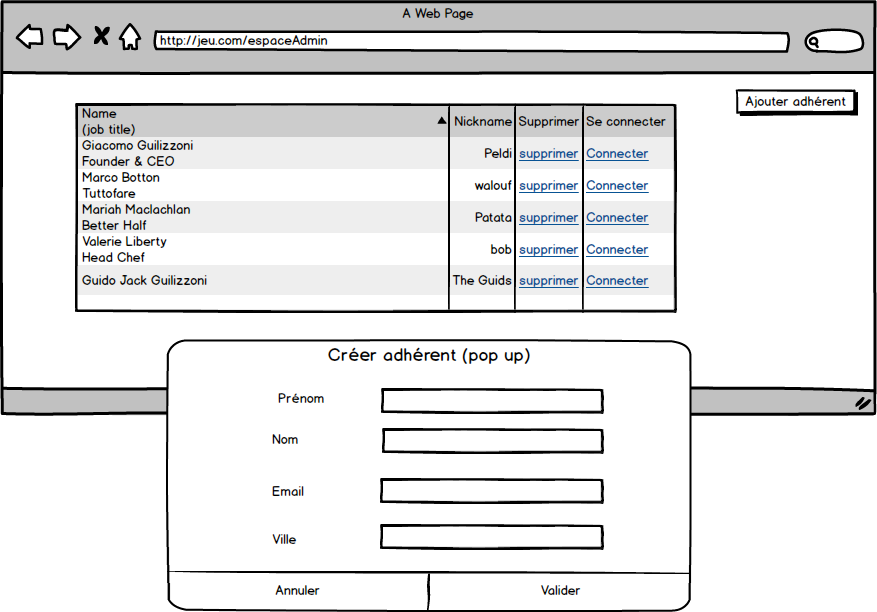
\includegraphics[width=350px]{../Maquette/espaceAdmin.png}
	\caption{Page d'administration par l'administrateur}
\end{figure}


\chapter{ Diagramme navigationnel}
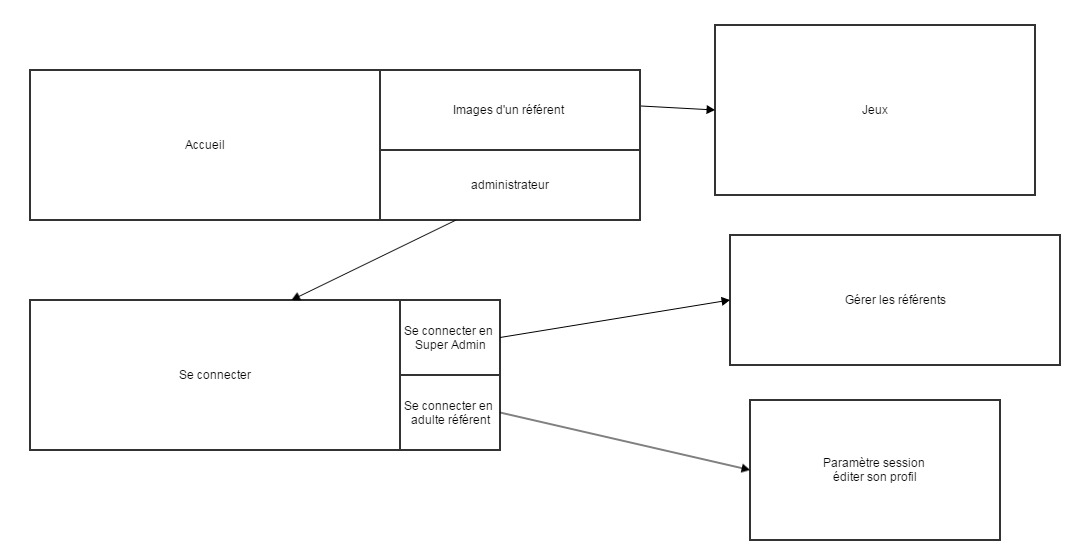
\includegraphics[width=350px]{../../UML/diagramme_navigationnel.jpg}\\

\chapter{Modèle Conceptuel}
\begin{figure}
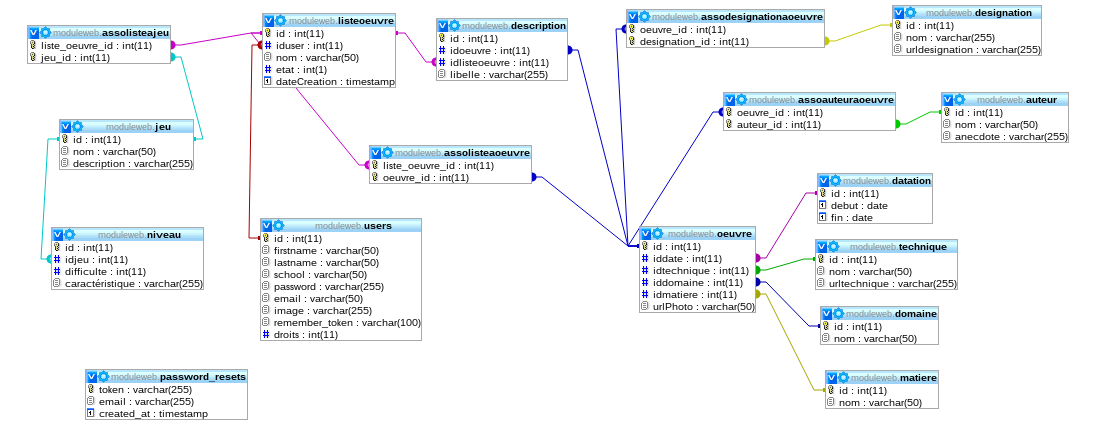
\includegraphics[width=450px]{../../UML/diagramClass2.png}\\
\end{figure}

\chapter{Liste et description traitement de donnée}
Traitement coté Client : 
Lorsque que l’on joue :\\
§  Les images des œuvres, leur titre et leur description sont chargées via AJAX au moment nécessaire (pré-chargement de l’image actuelle et de la suivante) puis sont associées aux jeux, développés en HTML5.
 
Lorsque l’on configure l’appli, partie Référent :\\
§  Les images sont affichées sous forme de miniatures sélectionnables.
§  On peut les associer à des groupes d’images, eux même pouvant être associés à des jeux. Les images seront sélectionnées via JavaScript.
 
Traitement coté Serveur :\\
·         Transformer les images en miniature.
·         Ajout des sons en « text-to-speech » et enregistrés sur le serveur dès l’ajout d’un titre d’œuvre.
·         Gestion des e-mails automatiques.

\chapter{Démarche test}
Démarche : \\
->Création, modification et suppression de compte référent par l'administrateur.\\
->Vue et modification des ses informations par un référents.\\
->Création de groupe d'œuvres en tant que référents. \\
->Test des différents jeux\\
->Modification et suppression de groupe d'œuvres par l'administrateur.\\
->Vérification des failles de sécurité avec un outil adapté.

\end{document}
